\chapter{Equilibrios ácido--base y método de la reacción predominante}\label{ch:b1:predominant-reaction}

El vinagre disuelve la cal de un hervidor; el zumo de limón también, un
poco más deprisa. La sangre mantiene su pH entre límites estrechos coma
lo que se coma; un refresco con gas es ácido por el dióxido de carbono
disuelto en él. Todos estos son equilibrios ácido--base en el agua, y un
químico ante una disolución que contiene varios ácidos y bases --- una
mezcla, un tampón, un \omterm{def:b1:predominant-reaction:polyprotic}{ácido poliprótico} --- necesita una manera fiable de
hallar su pH y las concentraciones de sus especies. Este capítulo
construye ese método: una escala de fuerzas, \omterm{def:b1:predominant-reaction:predominance}{diagramas de predominio} y el
\emph{método de la \omterm{def:b1:predominant-reaction:predominant-reaction}{reacción predominante}}, que reduce cualquier mezcla a
la única reacción que importa.

\begin{recall}
El libro 1 (año 12) definió los ácidos y \omterm{def:b1:predominant-reaction:bronsted}{bases de Brønsted}, la \omterm{def:b1:predominant-reaction:acidity-constant}{constante
de acidez} $K_a$ y el $\mathrm{p}K_a$, el \omterm{def:b1:predominant-reaction:autoprotolysis}{producto iónico del agua} y el pH
de los ácidos y \omterm{def:b1:predominant-reaction:strong-acid}{bases fuertes}, y dibujó \omterm{def:b1:predominant-reaction:predominance}{diagramas de predominio}. El
\omterm{def:b1:extent-q-and-k:quotient}{cociente de reacción}, la constante de equilibrio y las \omterm{def:b1:extent-q-and-k:activity}{actividades} de los
solutos ($c/c^\circ$) y del disolvente (1) se definieron en el
\cref{ch:b1:extent-q-and-k}; en este capítulo, $c^\circ = \qty{1}{mol/L}$
no se escribe en los cocientes.
\end{recall}

\begin{omfigure}
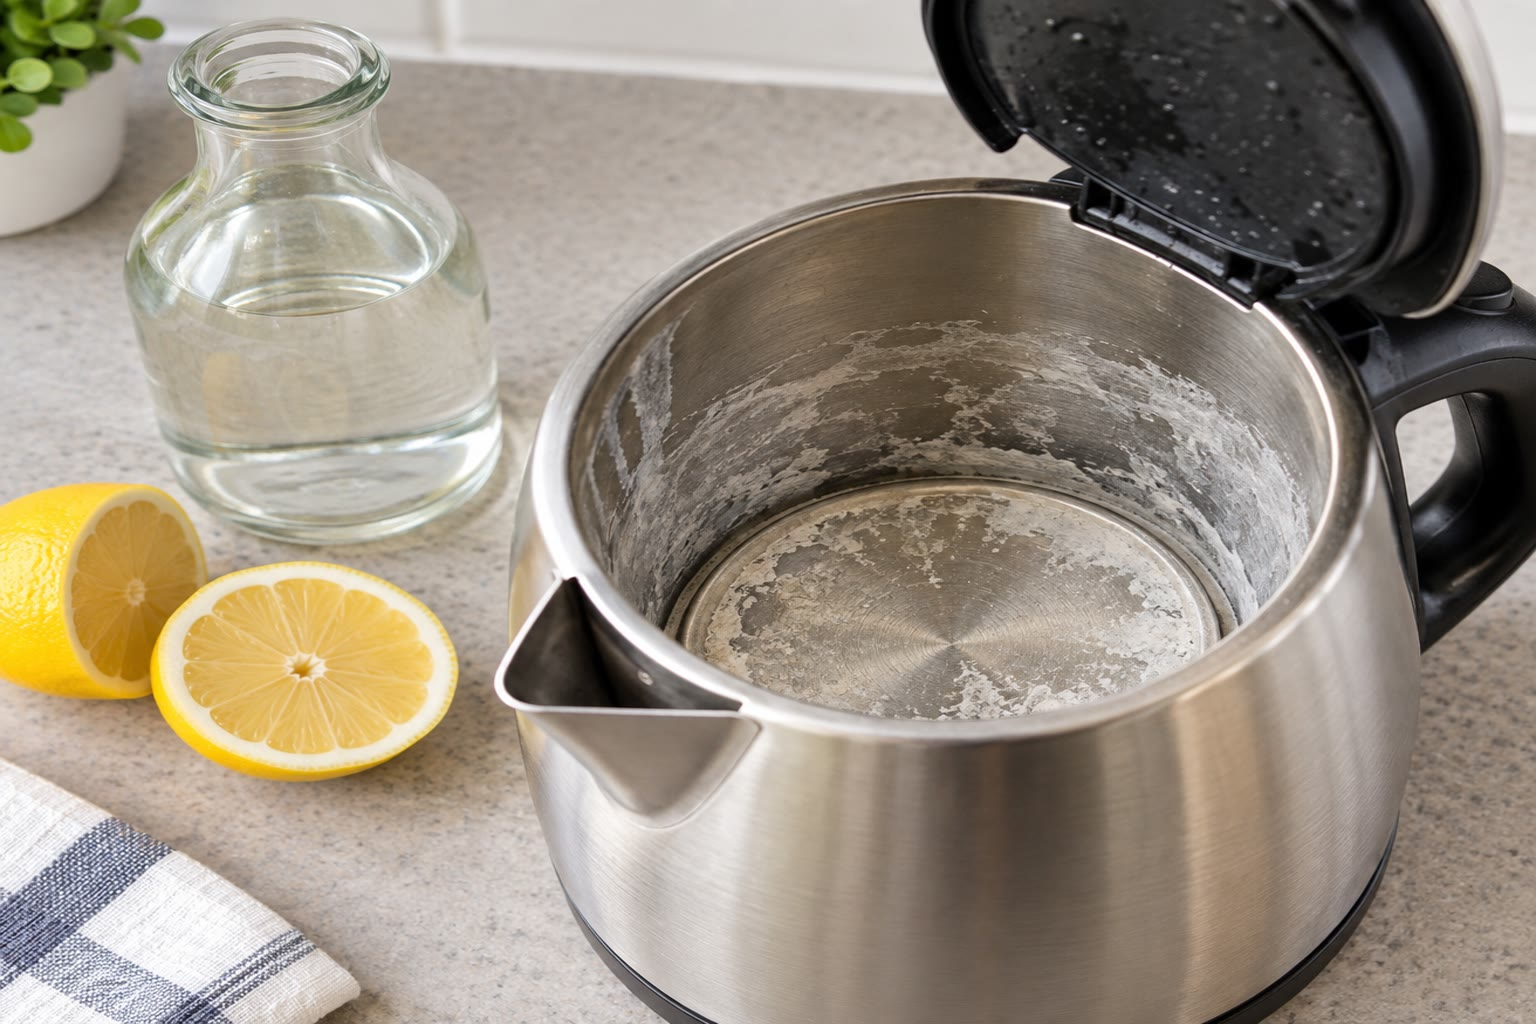
\includegraphics[width=0.5\linewidth]{images/book2/ai/b1-10-descaling.jpg}

{\small Cal, carbonato de calcio, en un hervidor. Los \omterm{def:b1:predominant-reaction:strong-acid}{ácidos débiles} del
vinagre y del zumo de limón reaccionan con el ion carbonato y la
disuelven.}
\end{omfigure}

\section{Pares de Brønsted y pH}

\begin{definition}[Ácido y base de Brønsted, par]\label{def:b1:predominant-reaction:bronsted}
Un \emph{ácido de Brønsted}\index{acido de Bronsted@ácido de Brønsted} es una especie capaz de
ceder un protón \ce{H+}; una \emph{base de Brønsted}\index{base de Bronsted@base de Brønsted} es
una especie capaz de captarlo. Un ácido HA y la base A en la que se
convierte al perder un protón forman un \emph{par ácido--base}\index{par acido--base@par ácido--base}
HA/A, relacionados por la semiecuación formal $\mathrm{HA} \rightleftharpoons
\mathrm{A} + \ce{H+}$. En el agua, el protón nunca está libre: lo
transporta una molécula de agua en forma de \ce{H3O+}.
\end{definition}

\begin{definition}[Anfolito]\label{def:b1:predominant-reaction:ampholyte}
Un \emph{anfolito}\index{anfolito} (una especie anfótera) es la base de un
par y el ácido de otro: el agua (\ce{H3O+}/\ce{H2O} y \ce{H2O}/\ce{OH-}),
el ion hidrogenocarbonato (\ce{CO2,H2O}/\ce{HCO3-}
y \ce{HCO3-}/\ce{CO3^{2-}}), el ion dihidrogenofosfato.
\end{definition}

\begin{definition}[Autoprotólisis, producto iónico, pH]\label{def:b1:predominant-reaction:autoprotolysis}
El agua experimenta la \emph{autoprotólisis}\index{autoprotolisis@autoprotólisis},
\ce{2H2O <=> H3O+ + OH-}, de constante $K_e = [\ce{H3O+}][\ce{OH-}]$, el
\emph{producto iónico del agua}\index{producto ionico del agua@producto iónico del agua}; a
\qty{25}{\celsius}, $K_e = 10^{-14.00}$, de modo que $\mathrm{p}K_e = 14.00$.
El pH de una disolución es $\mathrm{pH} = -\log a(\ce{H3O+}) \approx -\log[\ce{H3O+}]$.
Una disolución es neutra cuando $[\ce{H3O+}] = [\ce{OH-}]$, es decir, a
$\mathrm{pH} = \mathrm{p}K_e/2 = 7.00$ a \qty{25}{\celsius}.
% ledger: dfg:H2O_l, dfg:OH-_ao (pKe computed in figdata/bachelor-1/aqueous-constants.py)
\end{definition}

\section{Fuerza: \texorpdfstring{$K_a$}{Ka}, \texorpdfstring{p$K_a$}{pKa} y efecto nivelador}

\begin{definition}[Constante de acidez]\label{def:b1:predominant-reaction:acidity-constant}
La \emph{constante de acidez}\index{constante de acidez} de un par HA/A es
la constante de la reacción del ácido con el agua,
\[
  \mathrm{HA} + \ce{H2O} \rightleftharpoons \mathrm{A} + \ce{H3O+}, \qquad
  K_a = \frac{[\mathrm{A}][\ce{H3O+}]}{[\mathrm{HA}]}, \qquad
  \mathrm{p}K_a = -\log K_a .
\]
Cuanto mayor es $K_a$ (cuanto menor es $\mathrm{p}K_a$), más fuerte es el
ácido y más débil su base conjugada.
\end{definition}

\begin{definition}[Ácidos y bases fuertes y débiles]\label{def:b1:predominant-reaction:strong-acid}
Un ácido es \emph{fuerte}\index{acido fuerte@ácido fuerte} en el agua si su reacción con el
agua es total: no queda ninguna molécula HA (ácidos clorhídrico, nítrico
y perclórico, primera acidez del ácido sulfúrico); en caso contrario, es
\emph{débil}\index{acido debil@ácido débil}. Una base es \emph{fuerte}\index{base fuerte}
si su reacción con el agua es total y da \ce{OH-} (hidróxidos, ion óxido,
alcóxidos), y \emph{débil}\index{base debil@base débil} en caso contrario.
\end{definition}

\begin{definition}[Efecto nivelador]\label{def:b1:predominant-reaction:levelling}
En el agua, todo ácido más fuerte que \ce{H3O+} reacciona totalmente para
dar \ce{H3O+}, y toda base más fuerte que \ce{OH-}, totalmente para dar
\ce{OH-}: sus fuerzas no pueden distinguirse. Es el \emph{efecto
nivelador}\index{efecto nivelador} del disolvente. Los ácidos y \omterm{def:b1:predominant-reaction:strong-acid}{bases
débiles} en el agua tienen $0 < \mathrm{p}K_a < 14$; los pares del propio
agua ($\mathrm{p}K_a(\ce{H3O+}/\ce{H2O}) = 0$ y
$\mathrm{p}K_a(\ce{H2O}/\ce{OH-}) = 14$) limitan la escala.
\end{definition}

\begin{center}
\small
\begin{tabular}{lll@{\hspace{2.5em}}lll}
\hline
par & p$K_a$ & & par & p$K_a$ & \\
\hline
\ce{HSO4-}/\ce{SO4^{2-}} & 1.99 & & \ce{CO2,H2O}/\ce{HCO3-} & 6.37 & \\
\ce{H3PO4}/\ce{H2PO4-} & 2.15 & & \ce{H2PO4-}/\ce{HPO4^{2-}} & 7.21 & \\
\ce{HF}/\ce{F-} & 3.16 & & \ce{HClO}/\ce{ClO-} & 7.55 & \\
\ce{HCOOH}/\ce{HCOO-} & 3.74 & & \ce{NH4+}/\ce{NH3} & 9.25 & \\
\ce{CH3COOH}/\ce{CH3COO-} & 4.76 & & \ce{C6H5OH}/\ce{C6H5O-} & 9.99 & \\
\ce{C6H5NH3+}/\ce{C6H5NH2} & 4.60 & & \ce{HCO3-}/\ce{CO3^{2-}} & 10.33 & \\
\ce{C6H5COOH}/\ce{C6H5COO-} & 4.21 & & \ce{CH3NH3+}/\ce{CH3NH2} & 10.66 & \\
\hline
\end{tabular}
\end{center}
% ledger: pka:methanoic, pka:ethanoic, pka:anilinium, pka:benzoic,
% pka:phenol, pka:methylammonium (IUPAC dataset); dfg:HSO4-_ao,
% dfg:SO42-_ao, dfg:H3PO4_ao, dfg:H2PO4-_ao, dfg:HPO42-_ao, dfg:HF_ao,
% dfg:F-_ao, dfg:CO2_ao, dfg:HCO3-_ao, dfg:CO32-_ao, dfg:HClO_ao,
% dfg:ClO-_ao, dfg:NH4+_ao, dfg:NH3_ao (pKa computed from NBS-82)

\section{Diagramas de predominio y de distribución}

\begin{definition}[Diagramas de predominio y de distribución]\label{def:b1:predominant-reaction:predominance}
Para un par HA/A, $\mathrm{pH} = \mathrm{p}K_a + \log([\mathrm{A}]/[\mathrm{HA}])$:
predomina el ácido ($[\mathrm{HA}] > [\mathrm{A}]$) para
$\mathrm{pH} < \mathrm{p}K_a$, y la base para $\mathrm{pH} > \mathrm{p}K_a$.
El \emph{diagrama de predominio}\index{diagrama de predominio} es el eje
de pH dividido en cada $\mathrm{p}K_a$ en los dominios en los que
predomina cada forma. El \emph{diagrama de distribución}\index{diagrama de distribucion@diagrama de distribución}
da la fracción de cada forma, $[\text{forma}]/C$, en función del pH.
\end{definition}

\begin{proposition}[La relación de Henderson y las fracciones]\label{prop:b1:predominant-reaction:henderson}
Para un par HA/A de concentración total $C = [\mathrm{HA}] + [\mathrm{A}]$,
\[
  \mathrm{pH} = \mathrm{p}K_a + \log\frac{[\mathrm{A}]}{[\mathrm{HA}]}, \qquad
  \frac{[\mathrm{HA}]}{C} = \frac{1}{1 + 10^{\mathrm{pH} - \mathrm{p}K_a}}, \qquad
  \frac{[\mathrm{A}]}{C} = \frac{1}{1 + 10^{\mathrm{p}K_a - \mathrm{pH}}} .
\]
A una unidad de pH del $\mathrm{p}K_a$, la forma minoritaria está por
debajo del 10\,\% del total; a dos unidades, por debajo del 1\,\%.
\end{proposition}

\begin{proof}
Se toma el logaritmo de $K_a = [\mathrm{A}][\ce{H3O+}]/[\mathrm{HA}]$.
Entonces, $[\mathrm{A}]/[\mathrm{HA}] = 10^{\mathrm{pH}-\mathrm{p}K_a}$, y al
dividir $[\mathrm{HA}]$ entre $[\mathrm{HA}] + [\mathrm{A}]$ se obtienen
las fracciones. En
$\mathrm{pH} = \mathrm{p}K_a + 1$, $[\mathrm{HA}]/C = 1/11 < 10\,\%$; en
$+2$, $1/101$.
\end{proof}

\begin{omfigure}
\begin{tikzpicture}
\begin{axis}[name=e,
  width=0.48\linewidth, height=5.2cm, xmin=0, xmax=14, ymin=0, ymax=1.05,
  axis x line=bottom, axis y line=left, xlabel={pH}, ylabel={fracción},
  xtick={0,2,4,6,8,10,12,14},
  tick label style={font=\small}, label style={font=\small}]
\addplot[omDef, thick] table[x=pH, y=HA] {figdata/out/bachelor-1-distribution-diagrams-ethanoic.dat};
\addplot[omThm, thick] table[x=pH, y=A] {figdata/out/bachelor-1-distribution-diagrams-ethanoic.dat};
\draw[dotted] (axis cs:4.76,0) -- (axis cs:4.76,0.5);
\node[omDef, font=\footnotesize, anchor=west] at (axis cs:0.3,0.3) {\ce{CH3COOH}};
\node[omThm, font=\footnotesize, anchor=east] at (axis cs:13.7,0.3) {\ce{CH3COO-}};
\node[font=\small, anchor=north west] at (axis cs:4.8,0.48) {4.76};
\end{axis}
\begin{axis}[at={(e.east)}, anchor=west, xshift=1.1cm,
  width=0.48\linewidth, height=5.2cm, xmin=0, xmax=14, ymin=0, ymax=1.05,
  axis x line=bottom, axis y line=left, xlabel={pH}, ylabel={fracción},
  xtick={0,2,4,6,8,10,12,14},
  legend style={font=\scriptsize, draw=none, at={(0.5,1.04)}, anchor=south, legend columns=4},
  tick label style={font=\small}, label style={font=\small}]
\addplot[omDef, thick] table[x=pH, y=H3A] {figdata/out/bachelor-1-distribution-diagrams-phosphoric.dat};
\addplot[omMeth, thick] table[x=pH, y=H2A] {figdata/out/bachelor-1-distribution-diagrams-phosphoric.dat};
\addplot[omProp, thick] table[x=pH, y=HA] {figdata/out/bachelor-1-distribution-diagrams-phosphoric.dat};
\addplot[omThm, thick] table[x=pH, y=A] {figdata/out/bachelor-1-distribution-diagrams-phosphoric.dat};
\legend{\ce{H3PO4}, \ce{H2PO4-}, \ce{HPO4^{2-}}, \ce{PO4^{3-}}}

\end{axis}
\end{tikzpicture}

\begin{tikzpicture}[font=\small, >={Stealth}]
  \draw[->, thick] (0,0) -- (14.2*0.85,0) node[right] {pH};
  \foreach \x/\l in {2.15/2.15, 7.21/7.21, 12.34/12.34}
    \draw (\x*0.85,0.15) -- (\x*0.85,-0.15) node[below] {\l};
  \node[above] at (1.07*0.85,0.1) {\ce{H3PO4}};
  \node[above] at (4.68*0.85,0.1) {\ce{H2PO4-}};
  \node[above] at (9.78*0.85,0.1) {\ce{HPO4^{2-}}};
  \node[above] at (13.3*0.85,0.1) {\ce{PO4^{3-}}};
\end{tikzpicture}

{\small \omterm{def:b1:predominant-reaction:predominance}{Diagramas de distribución} del ácido etanoico (izquierda) y del
ácido fosfórico (derecha), y \omterm{def:b1:predominant-reaction:predominance}{diagrama de predominio} del ácido fosfórico.
Cada cruce de dos curvas vecinas está en un $\mathrm{p}K_a$; los
\omterm{def:b1:predominant-reaction:ampholyte}{anfolitos} \ce{H2PO4-} y \ce{HPO4^{2-}} son casi la única forma en el
centro de sus dominios.}
\end{omfigure}

\section{El método de la reacción predominante}

\begin{proposition}[Constante de una reacción ácido--base]\label{prop:b1:predominant-reaction:k-of-reaction}
La reacción del ácido $\mathrm{HA}_1$ de un par con la base
$\mathrm{A}_2$ de otro,
$\mathrm{HA}_1 + \mathrm{A}_2 \rightleftharpoons \mathrm{A}_1 + \mathrm{HA}_2$,
tiene la constante
\[
  K = \frac{K_{a1}}{K_{a2}} = 10^{\,\mathrm{p}K_{a2} - \mathrm{p}K_{a1}} .
\]
Es favorable ($K > 1$) cuando el ácido es más fuerte que el ácido que se
forma ($\mathrm{p}K_{a1} < \mathrm{p}K_{a2}$), y \omterm{def:b1:extent-q-and-k:quantitative}{cuantitativa} (en el
sentido del \cref{met:b1:extent-q-and-k:quantitative}) cuando la
diferencia de $\mathrm{p}K_a$ supera aproximadamente 4.
\end{proposition}

\begin{proof}
La reacción es la suma de $\mathrm{HA}_1 + \ce{H2O} \rightleftharpoons
\mathrm{A}_1 + \ce{H3O+}$ ($K_{a1}$) y de la inversa de $\mathrm{HA}_2 +
\ce{H2O} \rightleftharpoons \mathrm{A}_2 + \ce{H3O+}$ ($1/K_{a2}$);
la \cref{prop:b1:extent-q-and-k:combine-k} da $K = K_{a1}/K_{a2}$.
\end{proof}

\begin{definition}[Reacción predominante, disolución equivalente]\label{def:b1:predominant-reaction:predominant-reaction}
En una disolución que contiene varios ácidos y bases, la \emph{reacción
predominante}\index{reaccion predominante@reacción predominante} es la reacción de mayor constante
entre el ácido más fuerte y la base más fuerte presentes. Cuando es
\omterm{def:b1:extent-q-and-k:quantitative}{cuantitativa}, se trata como total, y la disolución se sustituye por la
\emph{disolución equivalente}\index{disolucion equivalente@disolución equivalente}: la disolución que
se obtiene una vez completada esta reacción, que tiene el mismo pH que la
real.
\end{definition}

\begin{method}[El método de la reacción predominante]\label{met:b1:predominant-reaction:method}
Para hallar el pH y la composición de una disolución:
\begin{enumerate}
  \item se enumeran las especies introducidas (y el agua) y se sitúan sus
        pares en una escala de $\mathrm{p}K_a$, los ácidos a un lado y las
        bases al otro;
  \item se buscan el ácido más fuerte y la base más fuerte presentes;
  \item si la constante de su reacción es grande ($K > 10^4$, o
        $\Delta\mathrm{p}K_a > 4$), se trata la reacción como total y se
        escribe la \omterm{def:b1:predominant-reaction:predominant-reaction}{disolución equivalente}; se vuelve al paso 2;
  \item cuando la \omterm{def:b1:predominant-reaction:predominant-reaction}{reacción predominante} tiene una constante pequeña, fija
        el pH: se escribe su tabla de avance y se resuelve $Q = K$,
        normalmente con la hipótesis de que su avance es pequeño;
  \item se comprueban las hipótesis: las especies minoritarias son
        efectivamente minoritarias, y las demás reacciones (incluida la
        \omterm{def:b1:predominant-reaction:autoprotolysis}{autoprotólisis} del agua) son despreciables.
\end{enumerate}
\end{method}

\begin{omfigure}
\begin{tikzpicture}[font=\small, >={Stealth}]
  \draw[->, thick] (0,-0.3) -- (0,7.6) node[above] {p$K_a$};
  \foreach \y/\a/\b in {0/\ce{H3O+}/\ce{H2O}, 1.58/\ce{HF}/\ce{F-}, 2.38/\ce{CH3COOH}/\ce{CH3COO-},
      3.62/\ce{H2PO4-}/\ce{HPO4^{2-}}, 4.62/\ce{NH4+}/\ce{NH3}, 7/\ce{H2O}/\ce{OH-}} {
    \draw (-0.12,\y) -- (0.12,\y);
    \node[anchor=east] at (-0.2,\y) {\a};
    \node[anchor=west] at (0.2,\y) {\b};
  }
  \foreach \y/\l in {0/0, 1.58/3.16, 2.38/4.76, 3.62/7.21, 4.62/9.25, 7/14} \node[black!60, anchor=west] at (3.0,\y) {\l};
  \draw[->, omThm, thick] (-1.6,2.55) -- (1.2,4.45);
  \node[omThm, anchor=west, align=left] at (4.2,3.5) {un ácido reacciona con cualquier\\base situada encima: $K > 1$};
  \node[anchor=south] at (-1.4,7.35) {ácidos};
  \node[anchor=south] at (1.2,7.35) {bases};
\end{tikzpicture}

{\small Una escala de $\mathrm{p}K_a$ (dibujada con el p$K_a$ creciente
hacia arriba; valores a la derecha). Un ácido reacciona favorablemente
con cualquier base situada encima de él en la escala: aquí, el ácido
etanoico con el amoniaco,
$K = 10^{9.25 - 4.76} = 10^{4.49}$.}
\end{omfigure}

\begin{proposition}[pH de disoluciones sencillas]\label{prop:b1:predominant-reaction:ph-formulas}
A la concentración $C$ (en \unit{mol/L}), con $\mathrm{p}C = -\log C$:
\begin{itemize}
  \item \omterm{def:b1:predominant-reaction:strong-acid}{ácido fuerte}: $\mathrm{pH} = \mathrm{p}C$, válido para
        $\mathrm{pH} < 6.5$;
  \item \omterm{def:b1:predominant-reaction:strong-acid}{ácido débil}, poco disociado: $\mathrm{pH} = \frac12(\mathrm{p}K_a
        + \mathrm{p}C)$, válido si $\mathrm{pH} < \mathrm{p}K_a - 1$;
  \item \omterm{def:b1:predominant-reaction:strong-acid}{base débil}, poco protonada: $\mathrm{pH} = \frac12(\mathrm{p}K_e +
        \mathrm{p}K_a - \mathrm{p}C)$, válido si $\mathrm{pH} > \mathrm{p}K_a +
        1$;
  \item \omterm{def:b1:predominant-reaction:ampholyte}{anfolito} con $\mathrm{p}K_{a2} - \mathrm{p}K_{a1} > 4$:
        $\mathrm{pH} = \frac12(\mathrm{p}K_{a1} + \mathrm{p}K_{a2})$,
        sea cual sea $C$ (si no es demasiado diluido).
\end{itemize}
\end{proposition}

\begin{proof}
\omterm{def:b1:predominant-reaction:strong-acid}{Ácido fuerte}: \ce{HA + H2O -> A- + H3O+} es total, $[\ce{H3O+}] = C$, y
la contribución del propio agua ($10^{-7}$) es despreciable si
$C > 10^{-6.5}$.
\omterm{def:b1:predominant-reaction:strong-acid}{Ácido débil}: la \omterm{def:b1:predominant-reaction:predominant-reaction}{reacción predominante} es $\mathrm{HA} + \ce{H2O}
\rightleftharpoons \mathrm{A} + \ce{H3O+}$, de avance $x = [\ce{H3O+}]
= [\mathrm{A}]$; si $x \ll C$, $K_a = x^2/C$, $\mathrm{pH} = \frac12(\mathrm{p}K_a
+ \mathrm{p}C)$; la hipótesis $[\mathrm{A}] < [\mathrm{HA}]/10$ es
$\mathrm{pH} < \mathrm{p}K_a - 1$. \omterm{def:b1:predominant-reaction:strong-acid}{Base débil}: lo mismo con $\mathrm{A} +
\ce{H2O} \rightleftharpoons \mathrm{HA} + \ce{OH-}$, de constante
$K_e/K_a$. \omterm{def:b1:predominant-reaction:ampholyte}{Anfolito} HA$^-$: la \omterm{def:b1:predominant-reaction:predominant-reaction}{reacción predominante} es
$2\,\mathrm{HA}^- \rightleftharpoons
\mathrm{H_2A} + \mathrm{A}^{2-}$, de modo que $[\mathrm{H_2A}] = [\mathrm{A}^{2-}]$;
al multiplicar $K_{a1} = [\mathrm{HA}^-]h/[\mathrm{H_2A}]$ por $K_{a2} =
[\mathrm{A}^{2-}]h/[\mathrm{HA}^-]$ se obtiene $h^2 = K_{a1}K_{a2}$.
\end{proof}

\begin{omfigure}
\begin{tikzpicture}
\begin{axis}[
  width=0.66\linewidth, height=5.6cm, xmin=0, xmax=8, ymin=0, ymax=8,
  axis x line=bottom, axis y line=left,
  xlabel={$\mathrm{p}C = -\log C$}, ylabel={pH},
  xtick={0,1,2,3,4,5,6,7,8}, ytick={0,1,2,3,4,5,6,7,8},
  tick label style={font=\small}, label style={font=\small},
  legend style={font=\small, draw=none, at={(0.02,0.98)}, anchor=north west}]
\addplot[omDef, very thick] table[x=pC, y=pH] {figdata/out/bachelor-1-weak-acid-ph.dat};
\addplot[omProp, dashed] table[x=pC, y=weak] {figdata/out/bachelor-1-weak-acid-ph.dat};
\addplot[black!50, dotted, thick] table[x=pC, y=strong] {figdata/out/bachelor-1-weak-acid-ph.dat};
\draw[black!30] (axis cs:0,7) -- (axis cs:8,7);
\legend{exacto, $\frac12(\mathrm{p}K_a + \mathrm{p}C)$, $\mathrm{pH} = \mathrm{p}C$}
\end{axis}
\end{tikzpicture}

{\small pH de disoluciones de ácido etanoico en función de $\mathrm{p}C$,
calculado exactamente a partir del balance de cargas. Concentrado, el
ácido está poco disociado y sigue $\frac12(\mathrm{p}K_a + \mathrm{p}C)$;
diluido por debajo de unos $10^{-6}$ mol/L, está totalmente disociado y se
comporta como un \omterm{def:b1:predominant-reaction:strong-acid}{ácido fuerte}; muy diluido, el pH tiende a 7.}
\end{omfigure}

\begin{example}[Ácido etanoico y amoniaco]\label{ex:b1:predominant-reaction:mixture}
Se mezclan \qty{0.10}{mol} de ácido etanoico y \qty{0.10}{mol} de amoniaco
en \qty{1.0}{L}. El ácido más fuerte es \ce{CH3COOH}, y la base más
fuerte,
\ce{NH3}: \ce{CH3COOH + NH3 <=> CH3COO- + NH4+}, $K = 10^{9.25 - 4.76} =
10^{4.49}$, \omterm{def:b1:extent-q-and-k:quantitative}{cuantitativa}. La \omterm{def:b1:predominant-reaction:predominant-reaction}{disolución equivalente} contiene
\qty{0.10}{mol/L} de \ce{CH3COO-} y de \ce{NH4+}. Su \omterm{def:b1:predominant-reaction:predominant-reaction}{reacción
predominante}, \ce{NH4+ + CH3COO- <=> NH3 + CH3COOH}, tiene la pequeña
constante $10^{-4.49}$ y mantiene $[\ce{NH3}] = [\ce{CH3COOH}]$, de donde,
como para un \omterm{def:b1:predominant-reaction:ampholyte}{anfolito}, $\mathrm{pH} = \frac12(4.76 + 9.25) = 7.01$.
\end{example}

\section{Ácidos polipróticos y tampones}

\begin{definition}[Ácido poliprótico]\label{def:b1:predominant-reaction:polyprotic}
Un \emph{ácido poliprótico}\index{acido poliprotico@ácido poliprótico} puede ceder
sucesivamente varios protones, cada etapa con su propia constante: el
ácido fosfórico \ce{H3PO4} ($\mathrm{p}K_a$ = 2.15, 7.21, 12.34), el
ácido carbónico (\ce{CO2,H2O}; 6.37, 10.33), el ácido sulfúrico (primera
acidez fuerte, segunda 1.99). Los $\mathrm{p}K_a$ sucesivos aumentan:
arrancar un protón a una especie que ya es negativa cuesta más.
\end{definition}

\begin{example}[Ácido fosfórico a \texorpdfstring{\qty{0.10}{mol/L}}{0.10 mol/L}]\label{ex:b1:predominant-reaction:h3po4}
La \omterm{def:b1:predominant-reaction:predominant-reaction}{reacción predominante} es la primera acidez. Con $x = [\ce{H3O+}]$,
$x^2/(0.10 - x) = 10^{-2.15}$; aquí $x$ no es pequeño frente a $C$, de
modo que se resuelve la ecuación de segundo grado
$x^2 + K_{a1}x - K_{a1}C = 0$: $x =
\qty{0.0233}{mol/L}$, $\mathrm{pH} = 1.63$. La segunda acidez
($\mathrm{p}K_{a2} = 7.21$) no contribuye en nada a este pH.
\end{example}

\begin{definition}[Disolución tampón]\label{def:b1:predominant-reaction:buffer}
Una \emph{disolución tampón}\index{disolucion tampon@disolución tampón} es una disolución cuyo
pH varía poco cuando se añade una pequeña cantidad de ácido o de base, o
cuando se diluye. El tampón habitual es una mezcla de un \omterm{def:b1:predominant-reaction:strong-acid}{ácido débil} y su
base conjugada en cantidades comparables; su pH es próximo al
$\mathrm{p}K_a$ del par.
\end{definition}

\begin{proposition}[Por qué resiste un tampón]\label{prop:b1:predominant-reaction:buffer}
Para un tampón de $n_a$ mol de ácido y $n_b$ mol de base,
$\mathrm{pH} =
\mathrm{p}K_a + \log(n_b/n_a)$ no depende del volumen. Añadir $\delta$
mol de un \omterm{def:b1:predominant-reaction:strong-acid}{ácido fuerte} lo modifica en
\[
  \Delta\mathrm{pH} = \log\frac{n_b - \delta}{n_a + \delta} - \log\frac{n_b}{n_a}
  \approx -\frac{\delta}{\ln 10}\left(\frac{1}{n_a} + \frac{1}{n_b}\right),
\]
que es mínimo para $n_a = n_b$ a cantidad total dada.
\end{proposition}

\begin{proof}
El \omterm{def:b1:predominant-reaction:strong-acid}{ácido fuerte} reacciona totalmente con la base: $n_b \to n_b - \delta$,
$n_a \to n_a + \delta$. La derivada de $f(\delta) = \log(n_b - \delta) -
\log(n_a + \delta)$ en 0 es $-\frac{1}{\ln10}\big(\frac{1}{n_b} +
\frac{1}{n_a}\big)$; con $n_a + n_b$ fijo, $\frac1{n_a} + \frac1{n_b}$ es
mínimo cuando $n_a = n_b$.
\end{proof}

\begin{definition}[Grado de disociación]\label{def:b1:predominant-reaction:dissociation}
El \emph{grado de disociación}\index{grado de disociacion@grado de disociación} de un \omterm{def:b1:predominant-reaction:strong-acid}{ácido
débil} HA a la concentración analítica $C$ es $\alpha = [\mathrm{A}]/C$, la
fracción del ácido disociada por el agua; cumple la ley de dilución de
Ostwald, $\alpha^2C/(1 - \alpha) = K_a$, y tiende a 1 cuando $C \to 0$.
\end{definition}

\begin{inthelab}[Preparar un tampón]
En el laboratorio, un tampón se prepara pesando el ácido y su sal (por
ejemplo, dihidrogenofosfato de sodio e hidrogenofosfato de disodio), o
añadiendo un volumen medido de disolución de hidróxido de sodio al ácido
mientras se lee un pHmetro, calibrado previamente con dos tampones
patrón; después se enrasa la disolución en un matraz aforado.
\end{inthelab}

\section{Ejercicios}

\begin{exercise}[$\star$]\label{exo:b1:predominant-reaction:1}
Escríbanse la base conjugada de \ce{H2SO4}, \ce{HCO3-}, \ce{NH4+} y
\ce{H2O}, y el ácido conjugado de \ce{NH3}, \ce{HPO4^{2-}}, \ce{OH-} y
\ce{H2O}. ¿Cuáles de estas especies son \omterm{def:b1:predominant-reaction:ampholyte}{anfolitos}?
\end{exercise}

\begin{exercise}[$\star$]\label{exo:b1:predominant-reaction:2}
Con la tabla de $\mathrm{p}K_a$, ordénense por su fuerza el ácido
fluorhídrico, el ácido etanoico, el ion amonio y el ácido hipocloroso, y
dese la $K_a$ de cada uno.
\end{exercise}

\begin{exercise}[$\star$]\label{exo:b1:predominant-reaction:3}
Calcúlese el pH de una disolución de ácido clorhídrico de
\qty{0.010}{mol/L} y el de una disolución de hidróxido de sodio de
\qty{0.010}{mol/L}, a \qty{25}{\celsius}.
\end{exercise}

\begin{exercise}[$\star$]\label{exo:b1:predominant-reaction:4}
Dibújese el \omterm{def:b1:predominant-reaction:predominance}{diagrama de predominio} del par \ce{CH3COOH}/\ce{CH3COO-}.
¿Qué forma predomina en un refresco de pH 3, y en la sangre, de pH 7.4?
¿Qué fracción del ácido está en forma ácida a pH 3.76?
\end{exercise}

\begin{exercise}[$\star\star$]\label{exo:b1:predominant-reaction:5}
Calcúlese el pH de una disolución de amoniaco de \qty{0.10}{mol/L} y
compruébese la hipótesis realizada.
\end{exercise}

\begin{exercise}[$\star\star$]\label{exo:b1:predominant-reaction:6}
Calcúlense el pH de una disolución de ácido etanoico de
\qty{0.010}{mol/L} y el \omterm{def:b1:predominant-reaction:dissociation}{grado de disociación}; compruébese la hipótesis.
\end{exercise}

\begin{exercise}[$\star\star$]\label{exo:b1:predominant-reaction:7}
Escríbanse la \omterm{def:b1:predominant-reaction:predominant-reaction}{reacción predominante}, su constante y el pH de una
disolución obtenida al mezclar, en \qty{1.0}{L}, \qty{0.10}{mol} de ácido
fluorhídrico y \qty{0.050}{mol} de hidróxido de sodio.
\end{exercise}

\begin{exercise}[$\star\star$]\label{exo:b1:predominant-reaction:8}
Un tampón contiene \qty{0.050}{mol} de ácido etanoico y \qty{0.050}{mol}
de etanoato de sodio en \qty{1.0}{L}. Calcúlese su pH y, después, el pH
tras añadir \qty{0.010}{mol} de ácido clorhídrico. Compárese con la misma
adición a \qty{1.0}{L} de agua pura.
\end{exercise}

\begin{exercise}[$\star\star$]\label{exo:b1:predominant-reaction:9}
Los ácidos clorhídrico y nítrico tienen la misma fuerza en el agua, pero
no en ácido etanoico puro como disolvente. Explíquese, y dígase cuál es
el ácido más fuerte que puede existir en el agua.
\end{exercise}

\begin{exercise}[$\star\star\star$]\label{exo:b1:predominant-reaction:10}
Calcúlese el pH de una disolución de carbonato de sodio de
\qty{0.10}{mol/L}, y compruébese que puede despreciarse la segunda
basicidad.
\end{exercise}

\begin{exercise}[$\star\star\star$]\label{exo:b1:predominant-reaction:11}
Demuéstrese la ley de dilución de Ostwald y calcúlese el \omterm{def:b1:predominant-reaction:dissociation}{grado de
disociación} del ácido etanoico a $C = \qty{1.0e-3}{mol/L}$. ¿Por qué falla
aquí la aproximación $\alpha \ll 1$?
\end{exercise}

\begin{exercise}[$\star\star\star$]\label{exo:b1:predominant-reaction:12}
Una disolución contiene \qty{0.010}{mol/L} de ácido clorhídrico y
\qty{0.10}{mol/L} de ácido etanoico. Hállense su pH y la concentración de
iones etanoato; explíquese por qué el \omterm{def:b1:predominant-reaction:strong-acid}{ácido débil} apenas se disocia.
\end{exercise}

\section{Problema: un tampón fosfato para el laboratorio de cultivo celular}

\begin{problem}[{Problema de fin de semana --- las tres acideces del ácido
fosfórico, el pH de sus tres sales de sodio, las disoluciones
equivalentes y el volumen de hidróxido de sodio que da un tampón de pH
7.20}]
\label{pb:b1:predominant-reaction:1}
Las células cultivadas en un laboratorio necesitan un medio de pH próximo
a 7.2. Datos a \qty{25}{\celsius}: $\mathrm{p}K_a$ del ácido fosfórico
2.15, 7.21 y
12.34; $\mathrm{p}K_e = 14.00$.

\medskip
\noindent\textbf{Parte I --- El ácido fosfórico.}
\begin{enumerate}
  \item Escríbanse los tres pares y sus semiecuaciones.
  \item Dibújese el \omterm{def:b1:predominant-reaction:predominance}{diagrama de predominio} del ácido fosfórico.
  \item ¿Qué especie predomina a pH 1, 5, 9 y 13?
  \item ¿Qué especies son \omterm{def:b1:predominant-reaction:ampholyte}{anfolitos}?
  \item ¿Por qué cada $\mathrm{p}K_a$ es mayor que el anterior?
\end{enumerate}

\medskip
\noindent\textbf{Parte II --- Tres disoluciones de \qty{0.100}{mol/L}.}
\begin{enumerate}[resume]
  \item Para el ácido fosfórico, escríbase la \omterm{def:b1:predominant-reaction:predominant-reaction}{reacción predominante} y
        demuéstrese que su avance no es despreciable frente a $C$.
  \item Calcúlese el pH de la disolución de ácido fosfórico.
  \item Para el dihidrogenofosfato de sodio \ce{NaH2PO4}, escríbanse la
        \omterm{def:b1:predominant-reaction:predominant-reaction}{reacción predominante} y su constante.
  \item Calcúlese el pH de esta disolución.
  \item Calcúlese el pH de una disolución de hidrogenofosfato de disodio
        \ce{Na2HPO4}.
  \item ¿Cuál de las tres disoluciones se acerca más al pH buscado?
\end{enumerate}

\medskip
\noindent\textbf{Parte III --- Adición de hidróxido de sodio.}
Una disolución contiene \qty{0.100}{mol} de \ce{H3PO4}; se añade
hidróxido de sodio, $n$ mol, con un volumen total de \qty{1.00}{L}.
\begin{enumerate}[resume]
  \item Escríbanse la reacción de los primeros \qty{0.100}{mol} de
        hidróxido y su constante. ¿Es \omterm{def:b1:extent-q-and-k:quantitative}{cuantitativa}?
  \item Descríbase la \omterm{def:b1:predominant-reaction:predominant-reaction}{disolución equivalente} para $n = \qty{0.100}{mol}$ y
        dese su pH.
  \item La misma pregunta para $n = \qty{0.150}{mol}$.
  \item La misma pregunta para $n = \qty{0.200}{mol}$.
  \item Esbócese el pH en función de $n$ de 0 a \qty{0.300}{mol}.
  \item ¿Por qué la disolución de la pregunta 14 es un buen tampón?
\end{enumerate}

\medskip
\noindent\textbf{Parte IV --- Preparar \qty{1.00}{L} de tampón de pH 7.20.}
Se dispone de hidróxido de sodio de \qty{1.00}{mol/L}.
\begin{enumerate}[resume]
  \item ¿Qué cociente $[\ce{HPO4^{2-}}]/[\ce{H2PO4-}]$ da pH 7.20?
  \item Exprésense las cantidades de \ce{H2PO4-} y de \ce{HPO4^{2-}} en
        función de la cantidad $x$ de hidróxido añadida más allá de los
        primeros \qty{0.100}{mol}.
  \item Calcúlese $x$.
  \item ¿Cuánto cambia el pH si se añaden \qty{1.0e-3}{mol} de ácido
        clorhídrico a este tampón? ¿Y a \qty{1.00}{L} de agua pura?
  \item ¿Cambiaría el pH si el tampón se diluyera diez veces?
        Explíquese.
  \item Calcúlese el volumen de disolución de hidróxido de sodio que hay
        que añadir a \qty{0.100}{mol} de ácido fosfórico para obtener
        \qty{1.00}{L} de tampón de pH 7.20.
\end{enumerate}
\end{problem}
